% --------------------------------------------------------------------------- %
\chapter{Appendix: Composing area\textasciitilde{}}
\markboth{}{Appendix: Composing area\textasciitilde{}}
% --------------------------------------------------------------------------- %

% --------------------------------------------------------------------------- %
\section{Related Media}
\begin{figure}[!ht]
    \centering
    \subcaptionbox{\rurl{youtu.be/SPd-f2EXuIQ}}[.3\linewidth]{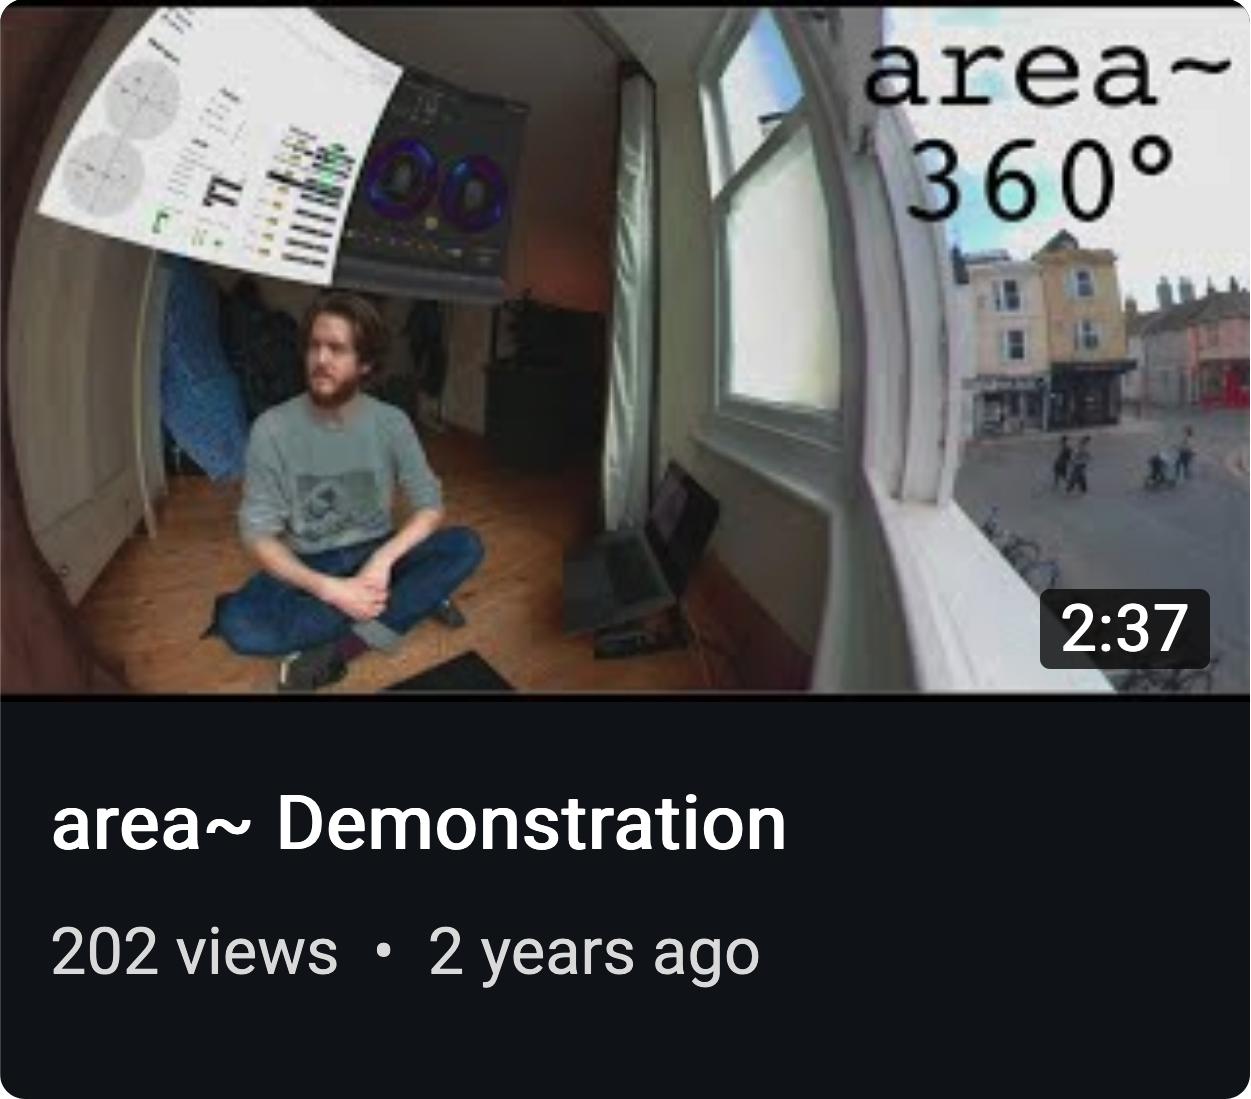
\includegraphics[height=4cm]{10-appendix-a/media/area-demonstration.png}}%
    \hfill
    \subcaptionbox{\rurl{youtu.be/rhtrAERxFQQ}}[.3\linewidth]{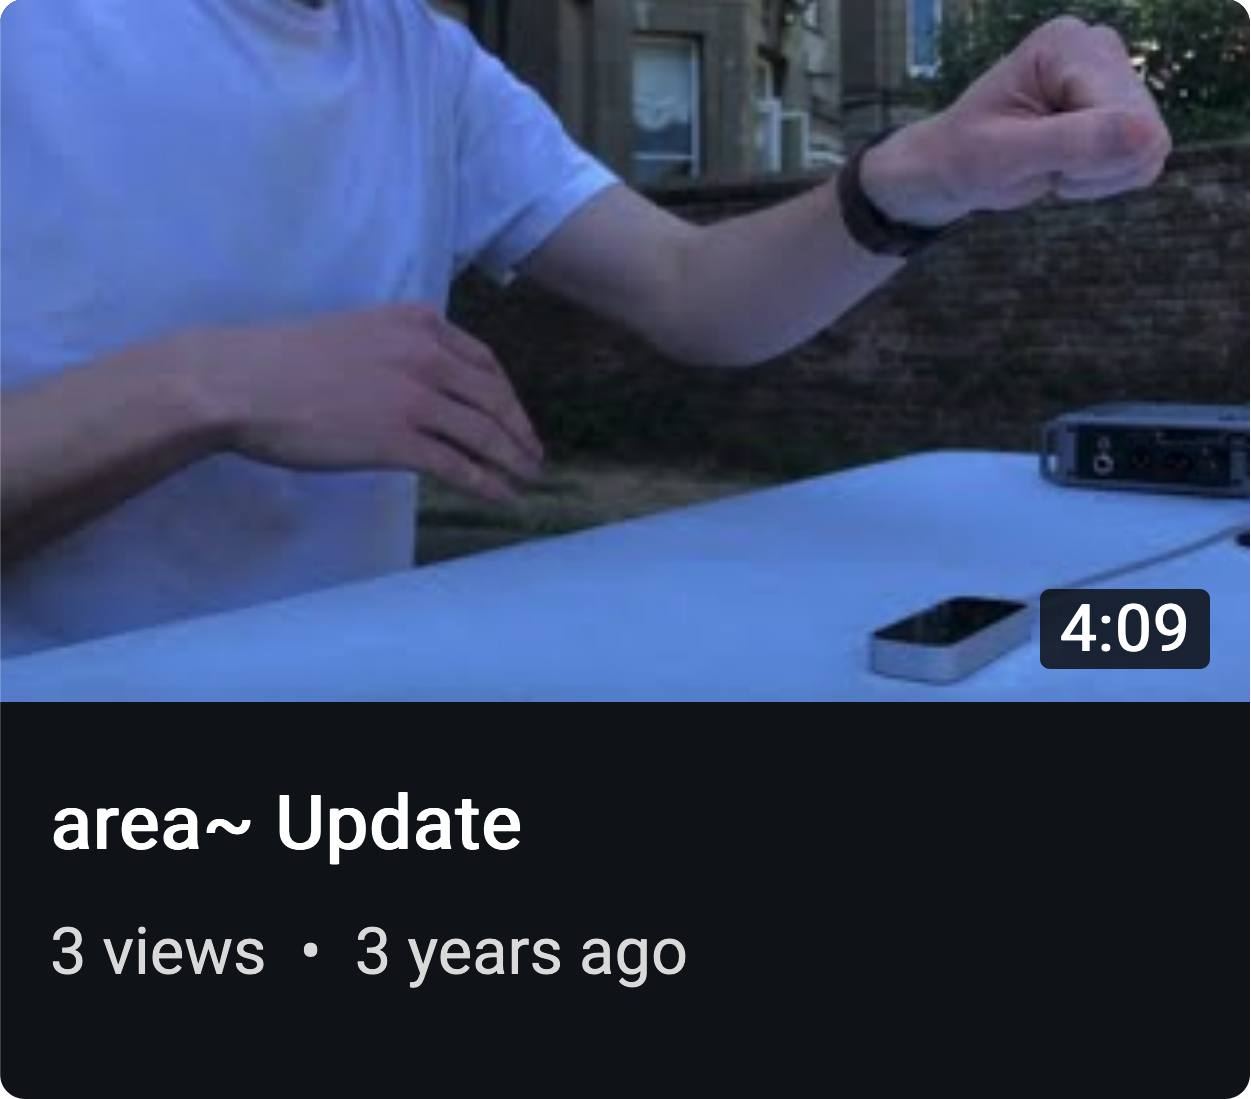
\includegraphics[height=4cm]{10-appendix-a/media/area-update.png}}
    \hfill
    \subcaptionbox{\centering \rurl{youtu.be/iZRcBhC13_4}}[.3\linewidth]{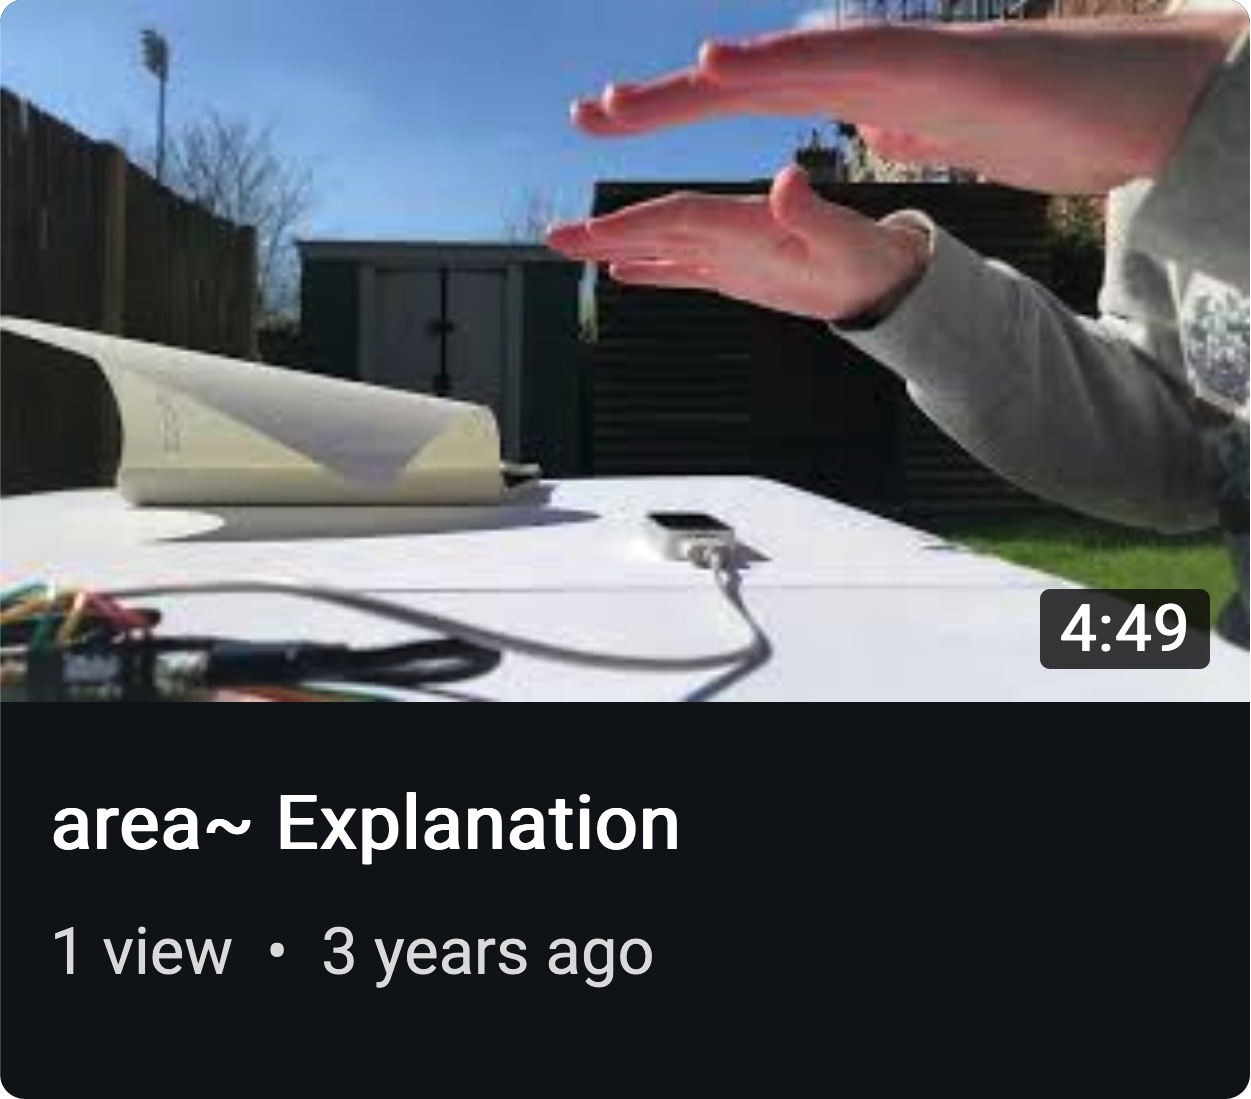
\includegraphics[height=4cm]{10-appendix-a/media/area-explanation.png}}
    \caption*{area\textasciitilde{} Video Recordings}
\end{figure}
\vspace*{1cm}
\begin{figure}[!ht]
    \centering
    \subcaptionbox*{\rurl{soundcloud.com/sambilbow/sets/area2020}}[0.6\linewidth]{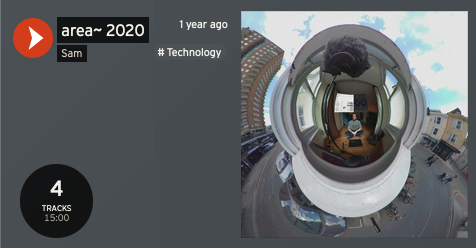
\includegraphics[height=4cm]{10-appendix-a/media/area-recordings}}
    \caption*{area\textasciitilde{} Binaural Audio Recordings}
\end{figure}
\clearpage



% --------------------------------------------------------------------------- %
\section{Code Repository}
\begin{figure}[!ht]
    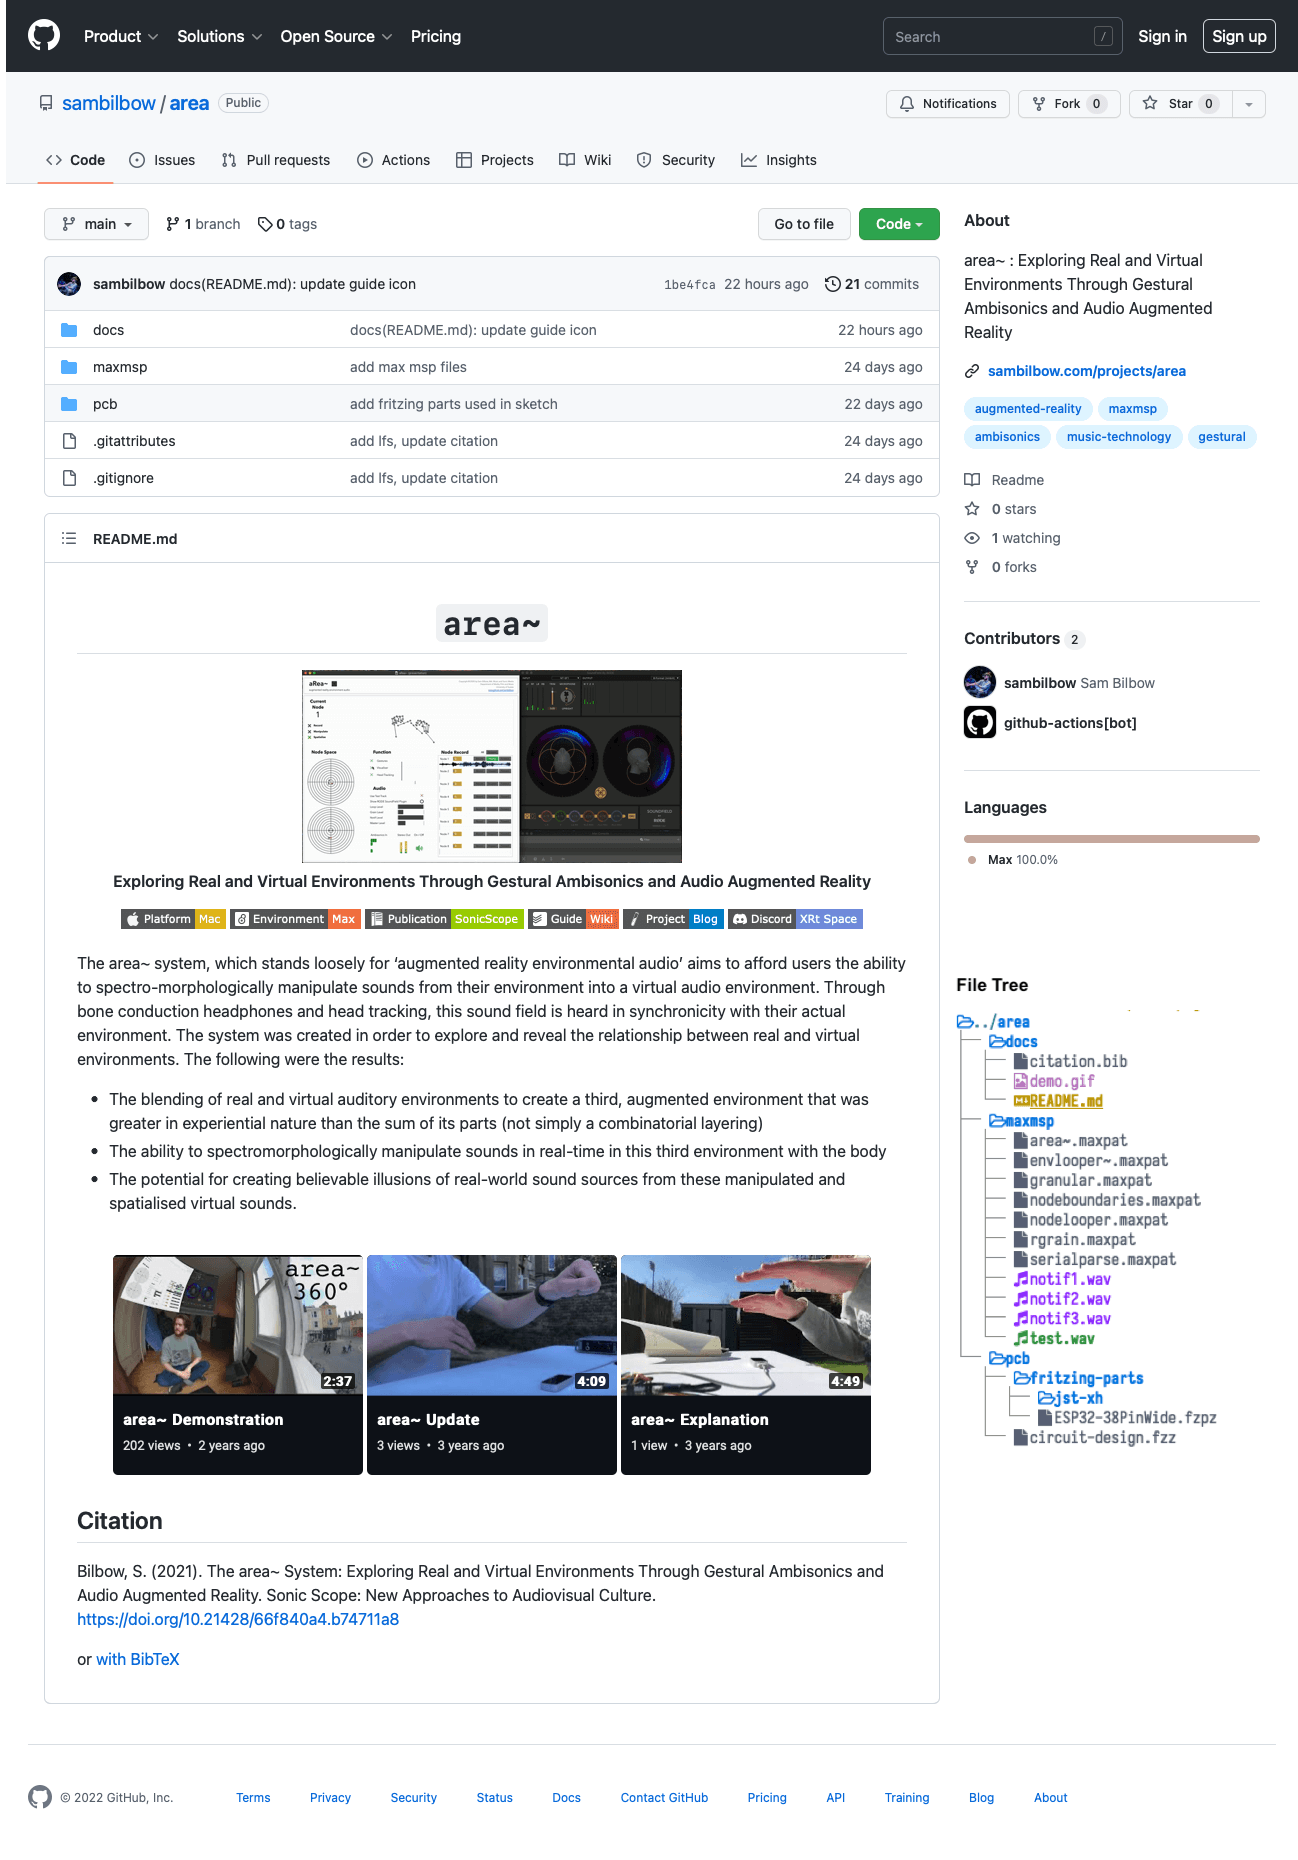
\includegraphics[width=\textwidth,height=\textheight,keepaspectratio]{10-appendix-a/area-code-file.png}
    \caption*{\rurl{github.com/sambilbow/area} \\ area\textasciitilde{} on GitHub with file tree}
\end{figure}
\clearpage



% --------------------------------------------------------------------------- %
% \section{Blog Contents}

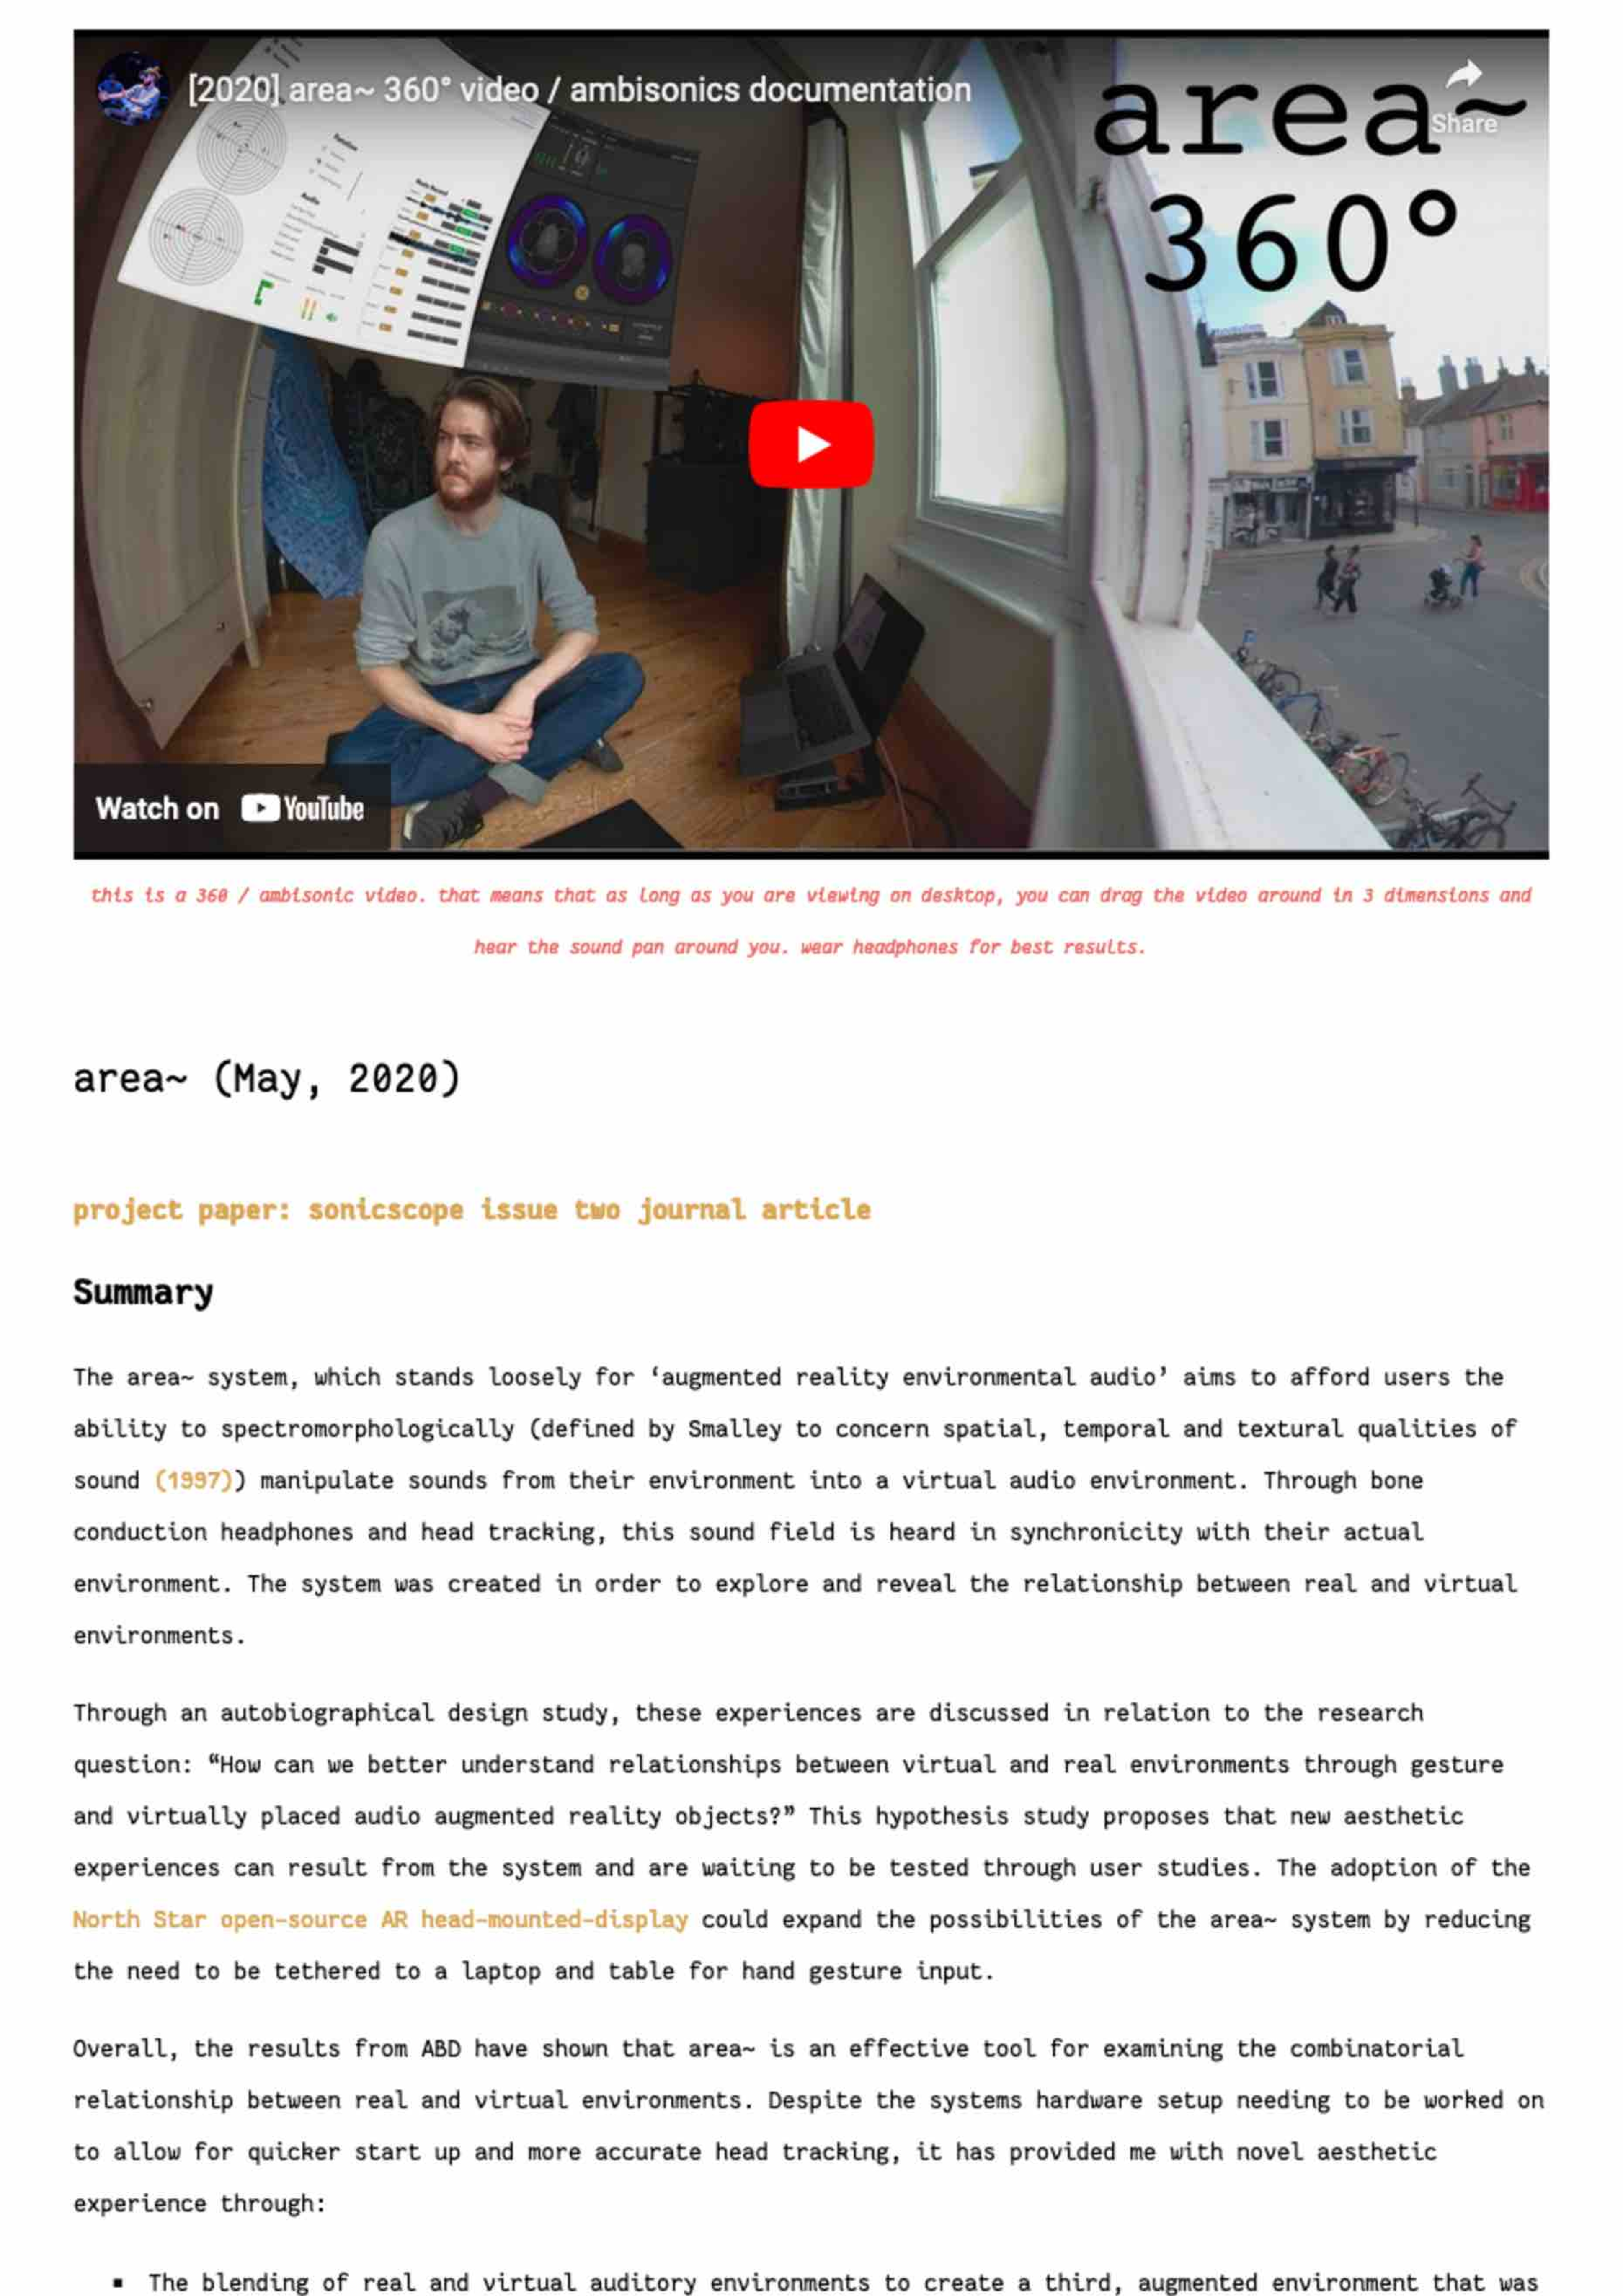
\includepdf[pages=1,pagecommand={\section{Blog Contents} \subsection{Summary}}, scale=0.71, frame, offset=10mm 0]{10-appendix-a/blog/summary.pdf}
\includepdf[pages=2-,pagecommand={}, scale=0.71, frame, offset=10mm 0]{10-appendix-a/blog/summary.pdf}



% --------------------------------------------------------------------------- %
\section{Project Guide}